\documentclass[11pt]{scrartcl}
\usepackage[sexy]{evan}
\usepackage{graphicx}
\usepackage[spanish]{babel}
\graphicspath{ {./images/} }

\usepackage{answers}
\Newassociation{hint}{hintitem}{all-hints}
\renewcommand{\solutionextension}{out}
\renewenvironment{hintitem}[1]{\item[\bfseries #1.]}{}

\usepackage{venndiagram,multicol,hyperref,graphicx,array,xskak}

\begin{document}
\title{Invarianza con restos}
\author{Ricardo Largaespada}
\date{15 Junio 2024}

\maketitle
\section{Introducción}

El concepto de invariantes es una herramienta poderosa en la resolución de problemas matemáticos, especialmente en aquellos que involucran operaciones repetitivas o transformaciones de estructuras. Un invariante es una propiedad que permanece constante a lo largo de una serie de operaciones o transformaciones. Cuando se trata de problemas que involucran restos (o residuos), los invariantes pueden ayudarnos a entender la estructura subyacente de un problema y a demostrar que ciertas condiciones se mantienen sin importar cuántas veces se apliquen ciertas operaciones.\\

En teoría de números, los restos son los resultados de la división de un número por otro, más específicamente el residuo cuando un número entero es dividido por otro número entero. Esta idea se formaliza en la aritmética modular. Por ejemplo, decir que dos números \( a \) y \( b \) son congruentes módulo \( n \) (escrito como \( a \equiv b \pmod{n} \)) significa que \( a \) y \( b \) dejan el mismo residuo cuando se dividen por \( n \).\\

Los invariantes con restos son particularmente útiles en problemas que involucran secuencias de números, operaciones repetitivas, y transformaciones en las cuales el módulo de un número juega un papel crucial. Al identificar un invariante con restos, podemos hacer afirmaciones fuertes sobre la imposibilidad o inevitabilidad de ciertas configuraciones o resultados finales.\\

Por ejemplo, si en un problema se puede demostrar que una cierta operación no cambia el residuo de un número respecto a un módulo dado, ese residuo es un invariante. Este tipo de razonamiento puede simplificar considerablemente la solución de problemas complejos.\\

En esta sección, exploraremos varios problemas que pueden ser resueltos usando invariantes con restos, mostrando cómo identificar estos invariantes y aplicarlos para llegar a conclusiones sobre las propiedades de los números involucrados y las operaciones permitidas.

\begin{example}
Un entero positivo está escrito en el tablero. Repetimos el proceso: borrar el dígito de las unidades y sumar 5 veces este dígito con el número restante. ¿Podemos, comenzando con \(7^{1998}\), terminar en \(1998^7\)?
\end{example}
Solución. Sea \( a_n \) el \( n \)-ésimo número de la lista. Escribimos este número de la siguiente forma \( a_n = 10t_n + u_n \), en que \( u_n \) es un dígito y \( t_n \) representa los primeros dígitos de \( a_n \). Por las condiciones dadas en el problema, debemos tener \( a_{n+1} = t_n + 5u_n \). Ahora, observe que \( t_n + 5u_n \equiv 50t_n + 5u_n \equiv 5(10t_n + u_n) \equiv 5a_n \pmod{7} \). Como \( a_1 = 7^{1998} \equiv 0 \pmod{7} \) y \( 1998^7 \not\equiv 0 \pmod{7} \), concluimos que es imposible que \(1998^7\) aparezca en la lista.

\begin{example}
Un número natural está escrito en el tablero. Siempre que el número \( x \) está escrito, podemos cambiarlo por \( 2x + 1 \) o por \( \frac{x}{x + 2} \). En algún momento, el número 2008 aparece en la lista. Demuestre que 2008 debe ser el primero.
\end{example}
Solución. Sea \( x = \frac{a}{b} \) un número racional escrito en su forma reducida. Defina la función \( f(x) = a + b \). Observe que:\begin{enumerate}
\item Si \( x' = 2x + 1 \), entonces \( x' = \frac{2a + b}{b} \). Como \( \gcd(2a + b, b) = \gcd(2a, b) \) por el lema de Euclides, entonces \( f(x') = 2f(x) \) o \( f(x') = f(x) \).
\item Si \( x' = \frac{x}{x + 2} = \frac{a}{a + 2b} \). Como \( \gcd(2b + a, b) = \gcd(2b, a) \) por el lema de Euclides, entonces \( f(x') \geq 2f(x) \) o \( f(x') = f(x) \).
\end{enumerate}

Como \( f(2008) = 2009 \), debe ser el primero.\\

\section{Semi-invariantes}
La idea de semi-invariante es una pequeña generalización de la idea de invariante. Diremos que una propiedad es semi-invariante cuando cambia de forma previsible (periódicamente, siempre creciendo o decreciendo). Un ejemplo bastante común de semi-invariante es la edad de una persona, que siempre crece de forma periódica (a cada 365 días).

\begin{example}
Nueve casillas \(1 \times 1\) de un tablero \(10 \times 10\) están infectadas. Cada segundo, una casilla que tiene dos casillas vecinas (con un lado en común) infectadas también se vuelve infectada. ¿Es posible que todas las casillas se vuelvan infectadas?
\end{example}

Solución. Veamos que una casa puede ser infectada de varias formas. Primero, vamos a analizar la siguiente ``infección'':

\begin{center}
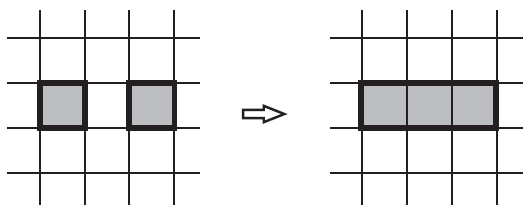
\includegraphics[width=0.3\textwidth]{images/clase_12_infeccion_tipo1.png}
\end{center}

Mirando la figura es fácil observar que el perímetro total del área infectada no cambia después de la infección del tipo 1. De este modo, podríamos pensar que este perímetro es invariante e igual a \(4 \times 9 = 36\). De ahí, como el perímetro de todo el tablero es \(4 \times 10 = 40\), sería imposible infectar completamente el tablero. Pero en este caso, estaríamos cometiendo un error grave: olvidar analizar todos los casos. Veamos qué pasa en los demás casos:

\begin{center}
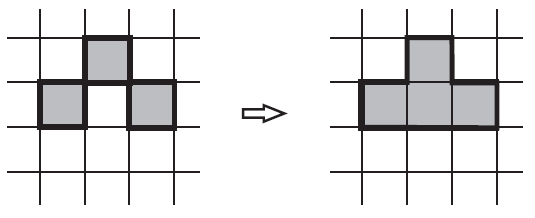
\includegraphics[width=0.3\textwidth]{images/clase_12_infeccion_tipo2.png}
\end{center}

Note que en este tipo de infección el perímetro no permanece constante, sino que disminuye en dos unidades. A primera vista esto puede parecer un problema, pero no lo es. Si el perímetro no aumenta, nunca podrá llegar a 40 (ya que inicialmente es como máximo 36). Sin embargo, para estar seguros de que esta hipótesis es verdadera, aún debemos analizar el último caso:

\begin{center}
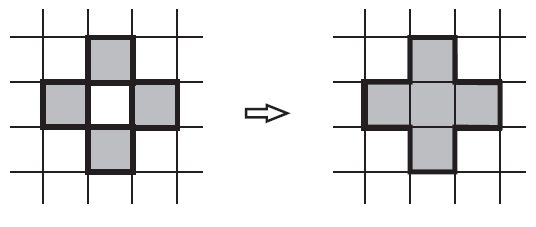
\includegraphics[width=0.3\textwidth]{images/clase_12_infeccion_tipo3.png}
\end{center}

Aquí podemos notar que el perímetro se hace aún menor, disminuyendo en cuatro unidades. Con esto, podemos concluir el problema. Es decir, ya que el perímetro inicial es como máximo 36 (en el caso en que no haya dos casillas infectadas vecinas) y nunca crece, jamás podremos infectar completamente el tablero.

\begin{example}
    Un total de 2000 personas están divididas entre los 115 cuartos de una mansión. Cada minuto, una persona se mueve a un cuarto con un número igual o mayor de personas que el cuarto del cual estaba. Demuestre que eventualmente todas las personas estarán en un mismo cuarto.
\end{example}
Solución. Sean \( a_1, a_2, \ldots, a_{115} \) la cantidad de personas en los cuartos 1, 2, ..., 115 respectivamente en un dado momento. Defina \( I = a_1^2 + a_2^2 + \cdots + a_{115}^2 \). Digamos que una persona sale de un cuarto con \( n \) personas y va a un cuarto con \( m \) personas (\( m \geq n \)). La variación de \( I \) está dada por:

\[ \Delta I = ((m + 1)^2 + (n - 1)^2) - (m^2 + n^2) = 2(m - n + 1) > 0 \]

Así, cada vez que una persona cambia de cuarto, el valor de \( I \) crece. Sin embargo, sabemos que el valor de \( I \) no puede crecer indefinidamente pues el número de personas es finito. Es decir, en un dado momento \( I \) no podrá crecer más, esto solo ocurrirá cuando ninguna persona pueda cambiar de cuarto. Luego, todas ellas deberán estar en el mismo cuarto.

\Opensolutionfile{all-hints}

\section{Problemas Propuestos}

\begin{problem}
(Rusia 1998) Un número de cuatro dígitos está escrito en el pizarrón. Las operaciones permitidas son: sumar 1 a dos dígitos vecinos (si ninguno de ellos es 9), o restar 1 de dos dígitos vecinos (si ninguno de ellos es 0). ¿Es posible obtener 2002 a partir de 1234 realizando algunas operaciones?
\begin{hint}
Analiza los cambios en los dígitos individuales y su impacto en el número total.
\end{hint}
\end{problem}

\begin{problem}
(Torneo de las Ciudades) Todo miembro de una secuencia, comenzando desde el segundo, es igual a la suma del término anterior con la suma de sus dígitos. El primer número es 1. ¿Es posible que 123456 pertenezca a la secuencia?
\begin{hint}
Observa la evolución de la secuencia y cómo la suma de dígitos influye en los términos.
\end{hint}
\end{problem}

\begin{problem}
(Hong Kong 1997) Cinco números 1, 2, 3, 4, 5 están escritos en un pizarrón. Un estudiante puede borrar dos de los números \( a \) y \( b \) y escribir en su lugar \( a+b \) y \( ab \). ¿Después de algunas operaciones podemos obtener la quíntuple 21, 27, 64, 180, 540?
\begin{hint}
Considera las combinaciones posibles y el impacto de las operaciones en los valores de los números.
\end{hint}
\end{problem}

\begin{problem}
(Torneo de las Ciudades 1985) En la isla de Camelot viven 13 camaleones morados, 15 verdes y 17 amarillos. Cuando dos de colores distintos se encuentran, cambian simultáneamente al tercer color. ¿Podría darse la situación en la cual todos tengan el mismo color?
\begin{hint}
Estudia la paridad de los cambios de colores y su impacto en el número total de camaleones de cada color.
\end{hint}
\end{problem}

\begin{problem}
En una fábrica de tarjetas existen tres máquinas. La primera recibe una tarjeta \((a, b)\) y devuelve una tarjeta \((a+1, b+1)\). La segunda recibe una tarjeta \((2a, 2b)\) y devuelve una tarjeta \((a, b)\). La tercera recibe dos tarjetas \((a, b)\) y \((b, c)\) y devuelve la tarjeta \((a, c)\). Todas las máquinas también devuelven la(s) tarjeta(s) dada(s). ¿Es posible fabricar una tarjeta \((1, 1988)\) si inicialmente solo tenemos una tarjeta \((5, 19)\)?
\begin{hint}
Analiza las transformaciones posibles y cómo pueden aplicarse secuencialmente para alcanzar la tarjeta deseada.
\end{hint}
\end{problem}

\begin{problem}
Con la calculadora KPK-1991 podemos efectuar dos operaciones: (a) elevar un número al cuadrado; y (b) obtener de un número \( X \) de \( n \) dígitos (\( n > 3 \)) el número \( A + B \), donde \( A \) es el número formado por los tres últimos de \( X \) y \( B \) el número formado por los \( (n-3) \) dígitos de \( X \). ¿Podemos obtener el número 703 a partir de 604 usando esta calculadora?
\begin{hint}
Considera las propiedades de las operaciones permitidas y cómo pueden aplicarse en secuencia para transformar 604 en 703.
\end{hint}
\end{problem}

\begin{problem}
(Rusia 1998) Los números 19 y 98 están escritos en el pizarrón. Cada minuto, a uno de ellos se le suma 1 y el otro se eleva al cuadrado. ¿Es posible que los dos números se vuelvan iguales después de varias operaciones?
\begin{hint}
Observa las posibles secuencias de operaciones y cómo afectan la paridad y magnitud de los números.
\end{hint}
\end{problem}

\begin{problem}
(Rusia 1998) Tenemos un tablero \( n \times n \) (\( n > 100 \)) con \( n - 1 \) casillas iguales a 1 y el resto iguales a 0. Podemos elegir una casilla, restar 1 de ella y sumar 1 a las demás casillas que están en la misma fila y columna de esta. ¿Con esta operación, podemos hacer que todas las casillas del tablero se vuelvan iguales?
\begin{hint}
Analiza cómo la operación afecta la suma total de los valores de las casillas y busca posibles invariantes.
\end{hint}
\end{problem}

\begin{problem}
(Leningrado) Existen \( n \geq 2 \) números no nulos escritos en un pizarrón. Podemos elegir dos números \( a \) y \( b \) y cambiarlos por \( \frac{a+b}{2} \) y \( \frac{b-a}{2} \). Demuestra que después de hacer un movimiento no podemos obtener los números iniciales nuevamente.
\begin{hint}
Considera las propiedades de las transformaciones y cómo afectan la estructura de los números en el pizarrón.
\end{hint}
\end{problem}

\begin{problem}
(Ucrania 2000) Existen inicialmente \( n \) números 1 escritos en un pizarrón. En cada paso podemos borrar \( a \) y \( b \) y escribir el número \( \frac{ab\sqrt{2}}{a + b} \) en su lugar. Después de repetir esta operación \( n - 1 \) veces, demuestra que el último número escrito no puede ser menor que \( \frac{1}{\sqrt{n}} \).
\begin{hint}
Analiza la función objetivo y cómo la operación la afecta en cada paso.
\end{hint}
\end{problem}

\begin{problem}
(San Petersburgo 1998) Un total de 119 enanos viven en una aldea con 120 pequeñas casillas. Una casa se dice super-habitada si 15 enanos o más viven en ella. Cada día, los enanos de una casa super-habitada tienen una pelea y se mudan a otras casillas de la aldea. ¿Algún día, necesariamente se terminará esta situación?
\begin{hint}
Considera el comportamiento de las casillas super-habitadas y cómo afecta la distribución de los enanos a lo largo del tiempo.
\end{hint}
\end{problem}

\begin{problem}
(Rusia 1997) Tenemos una fila larga de vasos y \( n \) piedras en el vaso central (vaso 0). Los siguientes movimientos son permitidos:\\
Movimiento tipo A:
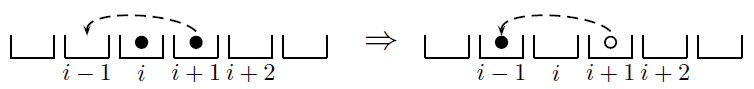
\includegraphics[width=12cm]{images/clase_12_cuerpo_1.png}

Si hay al menos una piedra en el vaso \( i \) y al menos una en el vaso \( i + 1 \), podemos hacer que una piedra que está en el vaso \( i + 1 \) salte al vaso \( i - 1 \) eliminando una piedra del vaso \( i \).\\

Movimiento tipo B:
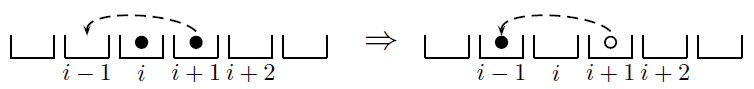
\includegraphics[width=12cm]{images/clase_12_cuerpo_1.png}
Si hay al menos dos piedras en el vaso \( i \), podemos saltar una piedra al vaso \( i + 2 \) y otra al vaso \( i - 1 \).

Demuestra el siguiente hecho: haciendo los movimientos tipo A o B durante un tiempo suficientemente largo, siempre llegamos a una configuración a partir de la cual no es posible hacer ninguno de estos dos tipos de movimiento. Además, esta configuración final no depende de la elección de movimientos durante el proceso.
\begin{hint}
Recuerda usar el concepto de energía para analizar las transformaciones.
\end{hint}
\end{problem}

\Closesolutionfile{all-hints}

\section{Sugerencias y Soluciones}
\begin{enumerate}
\input{all-hints.out}
\end{enumerate}

\end{document}